%Version 3.1 December 2024
% See section 11 of the User Manual for version history
%
%%%%%%%%%%%%%%%%%%%%%%%%%%%%%%%%%%%%%%%%%%%%%%%%%%%%%%%%%%%%%%%%%%%%%%
%%                                                                 %%
%% Please do not use \input{...} to include other tex files.       %%
%% Submit your LaTeX manuscript as one .tex document.              %%
%%                                                                 %%
%% All additional figures and files should be attached             %%
%% separately and not embedded in the \TeX\ document itself.       %%
%%                                                                 %%
%%%%%%%%%%%%%%%%%%%%%%%%%%%%%%%%%%%%%%%%%%%%%%%%%%%%%%%%%%%%%%%%%%%%%

%%\documentclass[referee,sn-basic]{sn-jnl}% referee option is meant for double line spacing

%%=======================================================%%
%% to print line numbers in the margin use lineno option %%
%%=======================================================%%

%%\documentclass[lineno,pdflatex,sn-basic]{sn-jnl}% Basic Springer Nature Reference Style/Chemistry Reference Style


%%\documentclass[sn-basic]{sn-jnl}% Basic Springer Nature Reference Style/Chemistry Reference Style

%%Note: the following reference styles support Namedate and Numbered referencing. By default the style follows the most common style. To switch between the options you can add or remove “Numbered” in the optional parenthesis. 
%%The option is available for: sn-basic.bst, sn-chicago.bst%  
 
%%\documentclass[pdflatex,sn-nature]{sn-jnl}% Style for submissions to Nature Portfolio journals
%%\documentclass[pdflatex,sn-basic]{sn-jnl}% Basic Springer Nature Reference Style/Chemistry Reference Style
\documentclass[iicol,sn-mathphys-num]{sn-jnl}% Math and Physical Sciences Numbered Reference Style
%%\documentclass[pdflatex,sn-mathphys-ay]{sn-jnl}% Math and Physical Sciences Author Year Reference Style
%%\documentclass[pdflatex,sn-aps]{sn-jnl}% American Physical Society (APS) Reference Style
%%\documentclass[pdflatex,sn-vancouver-num]{sn-jnl}% Vancouver Numbered Reference Style
%%\documentclass[pdflatex,sn-vancouver-ay]{sn-jnl}% Vancouver Author Year Reference Style
%%\documentclass[pdflatex,sn-apa]{sn-jnl}% APA Reference Style
%%\documentclass[pdflatex,sn-chicago]{sn-jnl}% Chicago-based Humanities Reference Style

%%%% Standard Packages
%%<additional latex packages if required can be included here>

\usepackage{graphicx}%
\usepackage{multirow}%
\usepackage{amsmath,amssymb,amsfonts}%
\usepackage{amsthm}%
\usepackage{mathrsfs}%
\usepackage[title]{appendix}%
\usepackage{xcolor}%
\usepackage{textcomp}%
\usepackage{manyfoot}%
\usepackage{booktabs}%
\usepackage{algorithm}%
\usepackage{algorithmicx}%
\usepackage{algpseudocode}%
\usepackage{subcaption}
\usepackage{listings}%
% \usepackage{fontspec} % Load the fontspec package
% \newfontfamily\hindifont{Noto Sans Devanagari}[Script=Devanagari] % Set script to Devanagari

%%%%

%%%%%=============================================================================%%%%
%%%%  Remarks: This template is provided to aid authors with the preparation
%%%%  of original research articles intended for submission to journals published 
%%%%  by Springer Nature. The guidance has been prepared in partnership with 
%%%%  production teams to conform to Springer Nature technical requirements. 
%%%%  Editorial and presentation requirements differ among journal portfolios and 
%%%%  research disciplines. You may find sections in this template are irrelevant 
%%%%  to your work and are empowered to omit any such section if allowed by the 
%%%%  journal you intend to submit to. The submission guidelines and policies 
%%%%  of the journal take precedence. A detailed User Manual is available in the 
%%%%  template package for technical guidance.
%%%%%=============================================================================%%%%

%% as per the requirement new theorem styles can be included as shown below
\theoremstyle{thmstyleone}%
\newtheorem{theorem}{Theorem}%  meant for continuous numbers
%%\newtheorem{theorem}{Theorem}[section]% meant for sectionwise numbers
%% optional argument [theorem] produces theorem numbering sequence instead of independent numbers for Proposition
\newtheorem{proposition}[theorem]{Proposition}% 
%%\newtheorem{proposition}{Proposition}% to get separate numbers for theorem and proposition etc.

\theoremstyle{thmstyletwo}%
\newtheorem{example}{Example}%
\newtheorem{remark}{Remark}%

\theoremstyle{thmstylethree}%
\newtheorem{definition}{Definition}%

\raggedbottom
%%\unnumbered% uncomment this for unnumbered level heads

\begin{document}

\title[Article Title]{EmotionFusion: A Deep Learning Approach to Speech Emotion Recognition}

%%=============================================================%%
%% GivenName	-> \fnm{Joergen W.}
%% Particle	-> \spfx{van der} -> surname prefix
%% FamilyName	-> \sur{Ploeg}
%% Suffix	-> \sfx{IV}
%% \author*[1,2]{\fnm{Joergen W.} \spfx{van der} \sur{Ploeg} 
%%  \sfx{IV}}\email{iauthor@gmail.com}
%%=============================================================%%

\author*[1]{\fnm{Shubham} \sur{Vankalas}}\email{svankalas1@gmail.com}

\author[1]{\fnm{Vandana} \sur{Dhingra}}\email{gotovandana@gmail.com}
\equalcont{These authors contributed equally to this work.}

\affil*[1]{\orgdiv{Department Of Technology}, \orgname{Savitribai Phule Pune University}, \orgaddress{\street{Ganeshkhind Rd}, \city{Pune}, \postcode{411007}, \state{Maharashtra}, \country{India}}}

% \affil[2]{\orgdiv{Department Of Technology}, \orgname{Savitribai Phule Pune University}, \orgaddress{\street{Ganeshkhind Rd}, \city{Pune}, \postcode{411007}, \state{Maharashtra}, \country{India}}}


%%==================================%%
%% Sample for unstructured abstract %%
%%==================================%%

\abstract{Speech is considered the most natural and efficient way of communicating and holds great potential for enabling seamless human-computer interaction. Yet, despite many advancements in semantic understanding, machines struggle to understand the emotional meaning of the spoken words. This paper proposes a deep learning approach for classifying emotions in Hindi and English speech by extracting acoustic features from the audio and sentiment from the speech content. The proposed method utilizes multiple datasets, consisting of Hindi and English corpora that are merged to create a diverse dataset. Data augmentation techniques such as noise injection and pitch bending are performed on these audio samples, improving the robustness of the classification process. Acoustic features such as Zero Crossing Rate (ZCR), Root Mean Square Energy (RMS), and Mel Frequency Cepstral Coefficients (MFCC) are crucial for recognizing emotions, as they capture meaningful characteristics and slight shifts in human speech. Alongside extracting acoustic features, we extracted sentiments from the speech using a pre-trained Hubert model, which provides insights into the linguistic content of the speech. We fuse these audio features and sentiments together before feeding them into the CNN-1D architecture. The proposed system achieved an accuracy of 96.56\%, which outperforms the results of recent relevant studies.}

\keywords{Speech emotion recognition, Deep learning, Acoustic features, Sentiment analysis, Feature fusion, Multilingual emotion recognition}

%%\pacs[JEL Classification]{D8, H51}

%%\pacs[MSC Classification]{35A01, 65L10, 65L12, 65L20, 65L70}

\maketitle

\section{Introduction}\label{sec1}

% \cite{r18}

Natural human-machine communication has long been an active area of research, with speech emerging as one of the most expressive and efficient modalities for interaction. While significant progress has been made in automatic speech recognition, the emotional dimension of spoken language remains a critical yet underexplored aspect of Human-Machine Interaction (HMI). Recognizing and responding to the emotional state of a speaker enables machines to move beyond passive command execution toward genuinely adaptive and context-aware communication. The practical implications of this capability are considerable — emotionally intelligent systems can enhance user experience across a wide range of applications, from virtual assistants that detect user frustration and adjust their responses accordingly, to affective computing systems that support mental health monitoring, personalized education, and empathetic customer service.

Despite significant advances driven by deep learning, existing Speech Emotion Recognition (SER) systems remain largely constrained by two key limitations: (i) a predominant focus on monolingual datasets, primarily English, which restricts their applicability in multilingual and low-resource settings, and (ii) an over-reliance on either handcrafted acoustic features or deep learned representations in isolation, limiting the ability to capture both low-level signal characteristics and high-level semantic context simultaneously.

A key observation motivating this work is that emotional expression in speech is not constrained by linguistic boundaries \cite{r20}. Paralinguistic cues such as changes in pitch, energy, and vocal rhythm convey emotional information independently of the language being spoken. This universality, however, does not imply uniformity. Languages such as Hindi, spoken by over 600 million people globally encode emotion through culturally distinct prosodic patterns, where subtle variations in tone and rhythm can substantially alter the intended meaning of an utterance. In real-world scenarios, speech signals are further characterized by variability in speaker traits, recording environments, and background noise. These challenges that are amplified in multilingual contexts such as Hindi–English speech, where differences in phonetics, prosody, and linguistic structure introduce additional complexity. Conventional models often exhibit reduced robustness under such conditions, highlighting the need for more generalized and adaptable architectures.

To address these limitations, this paper proposes a unified deep learning framework for multilingual SER that integrates both acoustic and semantic representations. The proposed method combines traditional low-level descriptors, including  Zero Crossing Rate (ZCR), Root Mean Square Energy (RMS), and Mel Frequency Cepstral Coefficients (MFCCs), with high-level contextual embeddings derived from a pre-trained HuBERT model. This multimodal feature fusion enables the model to jointly capture spectral–temporal dynamics and semantic emotional cues embedded in speech. Data augmentation strategies, including dynamic noise injection and random pitch shifting, are employed to simulate real-world acoustic variability and enhance model robustness. The classification backbone is implemented using a one-dimensional Convolutional Neural Network (1D-CNN), optimized with adaptive learning rate scheduling and early stopping to ensure stable convergence and improved generalization\cite{r23, r24} .

The proposed framework is evaluated on a large-scale multilingual dataset constructed by combining five benchmark corpora: the Crowdsourced Emotional Multimodal Actors Dataset (CREMA-D), the Ryerson Audio-Visual Database of Emotional Speech and Song (RAVDESS), the Toronto Emotional Speech Set (TESS), the Surrey Audio-Visual Expressed Emotion database (SAVEE), and a Hindi SER dataset \cite{r25, r26, r27, r28}. Comprising 15,362 raw audio samples  expanded to 61,448 following augmentation, the dataset spans diverse speakers, recording conditions, and emotional expressions, enabling comprehensive evaluation across seven emotion classes: anger, disgust, fear, happiness, neutrality, sadness, and surprise.

The main contributions of this work are summarized as follows:
\begin{enumerate}

 \item \textbf{Multilingual SER Framework:} A unified deep learning approach for emotion recognition across Hindi and English speech, directly addressing the gap in multilingual and low-resource SER research.
\item \textbf{Acoustic--Semantic Feature Fusion:} Integration of handcrafted acoustic features (ZCR, RMS, MFCC) with contextual embeddings from a pre-trained HuBERT model, enabling richer and more discriminative emotional representations.
\item \textbf{Robustness through Data Augmentation:} Incorporation of dynamic noise injection and pitch shifting techniques to improve model performance under real-world acoustic variability and unseen conditions.
\item \textbf{Large-Scale Multi-Dataset Evaluation:} Construction and evaluation on a combined dataset derived from CREMA-D, RAVDESS, TESS, SAVEE, and a Hindi speech corpus, ensuring linguistic diversity and generalizability across speakers and environments.

 \item \textbf{Efficient CNN-Based Architecture:} Design of a computationally efficient 1D-CNN model with adaptive optimization strategies, delivering stable convergence and strong generalization without excessive computational overhead.
\end{enumerate}
The remainder of this paper is structured as follows: Section 2 focuses on relevant work in SER. Section 3 describes the proposed method, detailing the data augmentation techniques, feature extraction pipeline and the trained model. Section 4 presents our experimental results and comparative analysis. Finally, Section 5 concludes this paper and outlines future research directions.

\section{Related Work}\label{sec2}

Advancement in computation methods and diversity in datasets has led to significant progress in speech emotion recognition (SER). Early studies highlight the importance of emotional models in building SER systems, where categorical and dimensional models were important. Categorical models classify emotions into separate groups such as anger, happiness, sadness, and neutral \cite{r5}, while the dimensional models portray emotions on continuous axes like valence, arousal and dominance \cite{r1}. Datasets like the Berlin Emotional Speech Database (EMODB) \cite{r4} and the Interactive Emotional Motion Capture (IEMOCAP) corpus \cite{r3} which supported by these categorical and dimensional models, influence them in database designing and feature selections. The process of selecting a dataset is very important, as it directly impacts the performance of the SER system. Datasets such as EMODB \cite{r4}, eNTERFACE \cite{r7}, and SUSAS \cite{r6} which are publicly available, are being widely used for system benchmarking purposes. However, difficulty still remains due to changes in recording environments, speaker characteristics and expressiveness of the emotions. For example, the RECOLA database \cite{r2} which captures multimodal interactions expressed in natural settings, indicates the need for realistic expressions of emotions. Also the Vera am Mittag (VAM) corpus \cite{r8}, it incorporates both audio and video modalities to simulate real-world interactions. Despite the applicability, there are certain restrictions, such as limited size and lack of diversity. Effort also needs to be taken to expand the culturally inclusive resources. 


The important step in the creation of SER is preprocessing; it optimizes the raw audio data for better feature extraction and classification. A common technique used in preprocessing is signal framing, where a continuous audio signal is segmented into fixed or variable lengths of overlapping frames, capturing temporal dynamics and eliminating prosodic variability  \cite{r4}\cite{r9}. Energy-based techniques, like integral value (IAV), are used to identify the voiced segments and non-voiced segments by adding a threshold to the audio signal energy. Recent studies also speak about noise-robust preprocessing, such as denoising autoencoders or adaptive filtering, to handle audio distortions in real-world environments \cite{r2}. As end-to-end processing is becoming more integrated into deep learning frameworks, preprocessing remains essential for tasks like voice activity detection (VAD) \cite{r6}. But challenges still remain in cross-lingual, where the preprocessing must adapt to diverse acoustic conditions \cite{r4}.


Feature extraction still remains a critical step in SER. These low-level descriptors are input for the model, forming the backbone of traditional approaches. Some commonly used features are Mel-frequency cepstral coefficients (MFCCs), Zero-crossing rate (ZCR), Pitch, Energy and Harmonic-to-noise ratio (HNR) \cite{r5}. These features capture spectral, prosodic, and temporal characteristics of the speech, which are then combined with statistical functions like mean and standard deviation for classification. Recent studies have explored deep learning techniques to automatically learn unique features. For example, long short-term memory (LSTM) networks have been employed to extract hierarchical representations from raw audio \cite{r3}.


Progress in computational methods and data availability has evolved Speech emotion recognition (SER) from traditional machine learning techniques to modern artificial neural networks. Gaussian mixture models (GMMs) \cite{r1}, and random forests \cite{r4},rests on custom features like Mel-frequency cepstral coefficients (MFCCs) and prosodic descriptors, but the earlier systems were dependent on support vector machines (SVMs) \cite{r5}. The execution of the above mentioned models was delimited in capturing temporal variations and context-specific details. Designs like convolutional neural networks (CNNs) \cite{r3}, long short-term memory networks (LSTMs) \cite{r7}, and hybrid models (e.g., CNN-LSTM) \cite{r6} happen to be a byproduct of deep learning revolutionized SER, allowing complete learning and commonality. For example, capturing localized spectral patterns and temporal dependencies \cite{r6},with selective attention has shown resilience in 1D CNNs, while collaborative methods combining CNNs and LSTMs increase the precision of the accumulations  of diversified feature representation \cite{r9}.A new framework has also been adopted, such as graph-based approaches, which help convert speech signals into statistical values \cite{r4}. Challenges such as variable-length speech segments and speech errors were taken into consideration by these methods.

Systems combine speech with textual information \cite{r8}, facial aspects \cite{r2}, or body function studies \cite{r10} which surpass single modal equivalents, as emotions can take various forms. For example, identifying basic emotions such as indecisiveness or humor has become easier by incorporating BERT-based text embeddings with CNN-extracted audio features, providing greater precision \cite{r8}. Likewise, by syncing multiple numbers of audio recordings with cardiovascular fluctuations and the electrical activity occurring on the skin, one could understand current emotions by using IoT-enabled smart wearable devices \cite{r10}. Methods like cross-modal focus mechanisms \cite{r6} and hierarchical alignment \cite{r2} have been used to solve difficulties arising due to spatial and multimodal imbalances, which are the primary causes that affect syncing of data from multiple fields, yet there exist certain limitations during their application in everyday life. Understanding, adapting and affordability have become the prime requirements of SER designs. Preprocessing cost can be decreased while moving data from source to destination, which consists of original audio recordings that directly deal with the development of features \cite{r3}. For example, skip connections and normalizing input to each layer when coupled with 2D-CNNs give greater accuracy on standard datasets such as EMO-DB and SAVEE \cite{r9}. In the meantime, improving recognition of highly sensitive words in chaotic circumstances can be done by incorporating transformer-based encoders with CNNs or LSTMs to solve dependencies in expression \cite{r8}. As technological advancements continue, some challenges, such as dataset bias, model overfitting, and computational costs, hinder widespread adoption. It is necessary to fill the spaces between theoretical knowledge and its practical applications with scalable platforms that incorporate transfer learning \cite{r7} and lightweight structures suited for cutting-edge technologies like quantized neural networks \cite{r10}.

There are a variety of metrics to evaluate the speech emotion recognition (SER), providing a comprehensive performance evaluation. There are some commonly used metrics, such as accuracy, precision, recall and F1-score, which together address the challenges faced by imbalanced datasets and multi-class classification \cite{r5}. The accuracy measures the percentage of accurately classified examples, but this can be misleading in the case of imbalanced classes where some emotions are more dominant than others. Precision indicates the ratio of true positives out of all the positive predictions; on the other hand, recall evaluates the ability to identify all relevant instances of a specific emotion. The harmonic mean of precision and recall is called the F1-score, which provides an evaluation score used to compare models \cite{r6}. Moreover, in SER studies, unweighted average recall (UAR) is frequently preferred to address the issue caused by the imbalanced class, which is solved by averaging recall across all the emotion classes \cite{r4}. There are some visual metrics like confusion matrices, which can be used to visualize the performance of each class, providing insights about misclassification patterns \cite{r8}. Some advanced evolution techniques include probabilistic measures like the concordance correlation coefficient (CCC), used to evaluate emotional dimensions like valence and arousal. Techniques like leave-one-speaker-out (LOSO) or leave-one-utterance-out (LOUO) are used to verify robustness and cross-validation. These strategies ensure that SER systems generalize across unseen speakers and diverse acoustic settings.

\section{Methodology}\label{sec3}

\begin{figure*}[t]
\centering
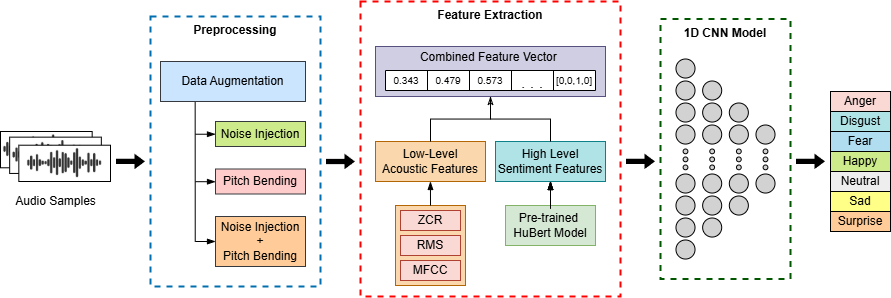
\includegraphics[width=\textwidth]{Paper Sys arch.png}
\caption{Proposed speech emotion recognition architecture}
\label{fig:system_architecture}
\end{figure*}


% This section explains the proposed framework shown in Figure \ref{fig:system_architecture}, that enabled our system for emotions recognizing. This framework first details the characteristics of the speech emotion datasets. We then discuss preprocessing, including data augmentation techniques that enhance robustness and generalization. Next, we'll explore the feature extraction pipeline that serves as input to our model. A deep dive into our model architecture and training process will follow. Finally, we'll outline evaluation metrics, such as accuracy and F1 score, to indicate the model's efficiency for our proposed emotion recognition system.

This section presents the overall methodology adopted for the proposed Speech Emotion Recognition (SER) framework. As illustrated in Fig. 1\ref {fig:system_architecture}, the pipeline consists of four key stages: dataset construction, preprocessing and data augmentation, feature extraction, and model design and training. The objective is to develop a robust multilingual SER system capable of capturing both acoustic and semantic characteristics of speech signals. Each component of the pipeline is carefully designed to enhance generalization and improve classification performance under diverse real-world conditions.

\subsection{Dataset}\label{subsec3.1}
The proposed framework utilizes a combination of publicly available benchmark datasets, including CREMA-D, RAVDESS, TESS, SAVEE,\cite{r25, r26, r27, r28} along with a Hindi speech emotion dataset. These datasets collectively provide a diverse set of speakers varying in gender, age, accent, and ethnicity, enabling the model to learn generalized emotional representations.

Since the emotional labels differ across datasets, a unified mapping strategy is employed to standardize all annotations into seven common emotion classes: anger, disgust, fear, happiness, neutrality, sadness, and surprise. This harmonization ensures consistency across datasets and facilitates effective multi-dataset training.


\subsubsection{Crowd-sourced Emotional Multimodal Actors Dataset (CREMA-D)}\label{subsubsec3.1.1}
\href{https://www.kaggle.com/datasets/ejlok1/cremad}
The CREMA-D is a widely used audio-visual dataset designed for studying multimodal emotional expression and perception. It contains recordings from 91 actors (48 male and 43 female) spanning an age range of 20 to 74 years and representing diverse ethnic backgrounds, including African American, Asian, Caucasian, and Hispanic groups.

The dataset comprises 7,442 clips recorded at a sampling rate of 48 kHz and includes three modalities: audio-only, visual-only, and audio-visual. In this work, only the audio modality is utilized to maintain consistency with the proposed SER framework. Each actor delivers a fixed set of 12 sentences under different emotional states.

The dataset includes six primary emotions—anger, happiness, sadness, fear, disgust, and neutrality—along with multiple intensity levels (low, medium, high, and unspecified). For consistency with the unified labeling scheme, these emotions are mapped to the standardized seven-class emotion set used in this study.

\subsubsection{Ryerson Audio-Visual Database of Emotional Speech and Song (RAVDESS)}\label{subsubsec3.1.2}
\href{https://www.kaggle.com/datasets/uwrfkaggler/ravdess-emotional-speech-audio}{Ryerson Audio-Visual Database of Emotional Speech and Song} (RAVDESS) The RAVDESS is a widely used multimodal dataset designed for the study of emotional expression in speech and song. It comprises recordings from 24 professional actors (12 male and 12 female), ensuring a balanced gender distribution. Each actor performs multiple lexically matched utterances in a neutral North American accent under controlled studio conditions.

The dataset includes both audio and video modalities, with a total of 7,356 recordings. In this study, only the audio modality is utilized, resulting in 1,440 speech recordings. The dataset captures eight emotional states: neutral, calm, happiness, sadness, anger, fear, surprise, and disgust, with two intensity levels (normal and strong) for all emotions except neutral. For consistency with the unified labeling scheme adopted in this work, these emotions are mapped to the standard seven-class emotion set.

\subsubsection{Hindi speech emotion recognition dataset}\label{subsubsec3.1.3}
\href{https://www.kaggle.com/datasets/vishlb/speech-emotion-recognition-hindi}{Hindi speech emotion recognition dataset}
The Hindi speech emotion dataset, developed by Vishal Bhardwaj, is specifically designed to facilitate emotion recognition in the Hindi language. The dataset consists of audio recordings of ten predefined Hindi sentences expressed across multiple emotional states.

It includes recordings from eight actors (four male and four female), each participating in five recording sessions. This results in approximately 3,200 audio samples. The dataset covers eight emotional categories: anger, disgust, fear, happiness, neutrality, sadness, sarcasm, and surprise. To maintain consistency across datasets, these labels are mapped to the standardized seven emotion classes used in this study.

\subsubsection{Toronto emotional speech set (TESS)}\label{subsubsec3.1.4}
\href{https://www.kaggle.com/datasets/ejlok1/toronto-emotional-speech-set-tess}{Toronto emotional speech set} (TESS) The TESS was developed at the University of Toronto to support research on emotion perception in speech. It contains high-quality audio recordings sampled at 24.414 kHz and provides a well-balanced distribution of emotional categories.

The dataset consists of 2,800 utterances spoken by two female actors aged 26 and 64 years, making it a gender-specific dataset. Each utterance corresponds to one of 200 target words embedded within a fixed carrier phrase (“Say the word”). The recordings express seven emotions: anger, disgust, fear, happiness, pleasant surprise, sadness, and neutrality. For consistency with the unified emotion framework, “pleasant surprise” is mapped to the “surprise” category.


\subsubsection{Surrey Audio-Visual Expressed Emotion database (SAVEE)}\label{subsubsec3.1.5}
\href{https://www.kaggle.com/datasets/ejlok1/surrey-audiovisual-expressed-emotion-savee}{Surrey Audio-Visual Expressed Emotion database} (SAVEE) The SAVEE dataset was developed by researchers at the University of Surrey to support studies in speech-based emotion recognition and human–computer interaction. It provides high-quality audio recordings sampled at 44.1 kHz and includes speech data from four male native British English speakers.

The dataset consists of recordings derived from 15 sentences selected from the TIMIT corpus, including three common sentences, two emotion-specific sentences, and ten phonetically balanced sentences tailored to different emotional expressions. To ensure consistency, the common and emotion-specific sentences were also recorded under neutral conditions, resulting in a total of 120 utterances per speaker and 480 audio samples overall.

The recordings capture seven emotional categories: anger, disgust, fear, happiness, sadness, surprise, and neutrality. In this study, only the audio modality is utilized, and the emotion labels are aligned with the standardized seven-class emotion framework adopted across all datasets.

\subsection{Preprocessing}\label{subsec3.2}
All publicly available speech emotion datasets were collected and merged into a unified dataset to facilitate consistent processing and analysis. This consolidation enables uniform label representation across datasets while providing a diverse set of speech samples. The combined dataset consists of 15,362 audio recordings, forming a comprehensive foundation for training the proposed model as shown in Tables 1 \ref{tab:emotion_distribution}, AND Table 2  \ref{tab:actors_per_dataset}and 2).

To ensure consistency in emotion labels across different datasets, an emotion harmonization strategy was employed. Specifically, all dataset-specific emotion categories were mapped to a standardized set of seven classes: anger, disgust, fear, happiness, neutrality, sadness, and surprise, as illustrated in Fig. 2 \ref{fig:final_count}. This step is essential due to variations in labeling conventions across datasets.

To enhance model robustness and generalization, several data augmentation techniques were applied to the training data. These include noise injection, pitch shifting, and a combination of both transformations. First, additive white noise was introduced with randomly varying intensity levels to simulate real-world acoustic disturbances. Next, pitch shifting was applied to modify the frequency characteristics of the audio signal without altering its temporal structure, thereby capturing natural variations in vocal tone. Finally, a combined augmentation strategy incorporating both noise and pitch modifications was applied to further increase variability.

Each original audio sample generated three augmented variants, while the original recordings were retained. As a result, the dataset size increased to 61,448 samples. All augmented samples preserved their corresponding emotion labels.

This augmentation strategy significantly improves the model’s ability to generalize across diverse acoustic environments and enhances robustness to noise and speaker variability. Fig. 3\ref{fig:surprise_audio_augmentation} presents representative waveform visualizations for the “surprise” emotion, demonstrating the impact of the applied augmentation techniques.


\begin{figure}[h]
\centering
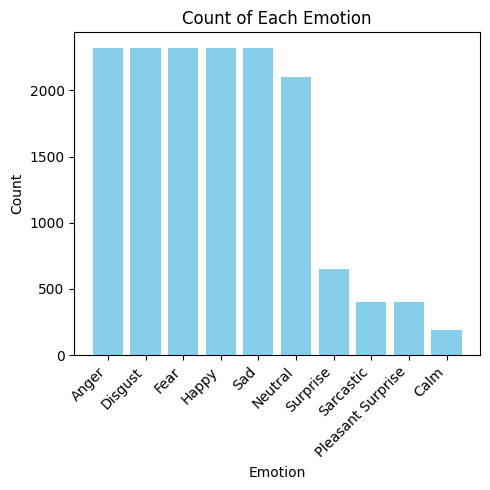
\includegraphics[width=\linewidth]{final count.png}
\caption{Count Plot of all emotions}
\label{fig:final_count}
\end{figure}

\begin{table*}[h]
\caption{Emotion Distribution by Dataset}\label{tab:emotion_distribution}%
\centering
\small
\begin{tabular}{@{}l|ccccc|c@{}}
\toprule
\textbf{Emotion} & \textbf{CREMA-D} & \textbf{RAVDESS} & \textbf{Hindi} & \textbf{TESS} & \textbf{SAVEE} & \textbf{Total} \\
\midrule
Anger & 1271 & 192 & 400 & 400 & 60 & 2323 \\
Disgust & 1271 & 192 & 400 & 400 & 60 & 2323 \\
Fear & 1271 & 192 & 400 & 400 & 60 & 2323 \\
Happy & 1271 & 192 & 400 & 400 & 60 & 2323 \\
Neutral & 1087 & 96 & 400 & 400 & 120 & 2103 \\
Sad & 1271 & 192 & 400 & 400 & 60 & 2323 \\
Calm & -- & 192 & -- & -- & -- & 192 \\
Surprise & -- & 192 & 400 & -- & 60 & 652 \\
Sarcastic & -- & -- & 400 & -- & -- & 400 \\
Pleasant Surprise & -- & -- & -- & 400 & -- & 400 \\
\midrule
\textbf{Total Samples} & 7442 & 1440 & 3200 & 2800 & 480 & \textbf{15362} \\
\bottomrule
\end{tabular}
\end{table*}

\begin{table*}[h]
\caption{Number of Actors per Dataset}\label{tab:actors_per_dataset}%
\centering
\small
\begin{tabular}{@{}l|ccccc@{}}
\toprule
\textbf{Actor Type} & \textbf{CREMA-D} & \textbf{RAVDESS} & \textbf{Hindi} & \textbf{TESS} & \textbf{SAVEE} \\
\midrule
Female Actors & 43 & 12 & 4 & 2 & - \\
Male Actors & 48 & 12 & 4 & 0 & - \\
\midrule
Total Actors & 91 & 24 & 8 & 2 & - \\
\bottomrule
\end{tabular}
\end{table*}

\begin{figure}[H]
    \centering
    % First row
    \begin{subfigure}[t]{0.48\textwidth} 
        \centering
        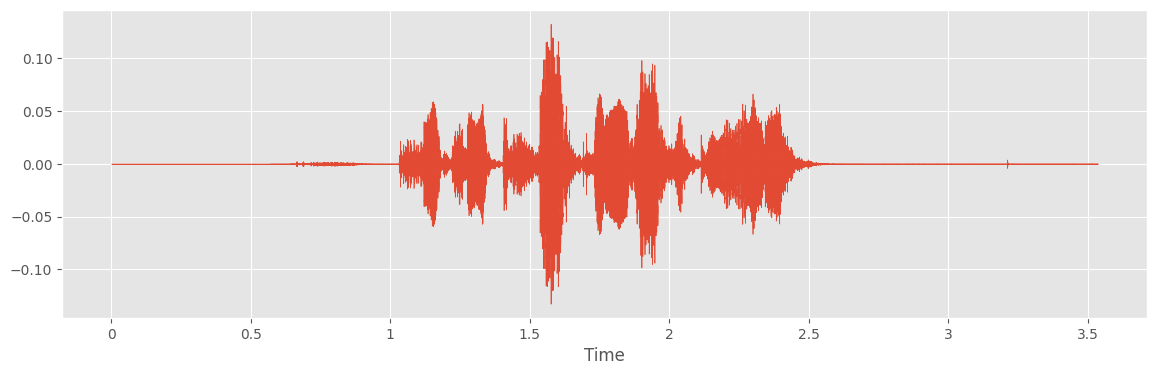
\includegraphics[width=\linewidth]{OG Surprise.png}
        \caption{Original audio waveform}
        \label{fig:surprise_og}
    \end{subfigure}\hfill
    \begin{subfigure}[t]{0.48\textwidth}
        \centering
        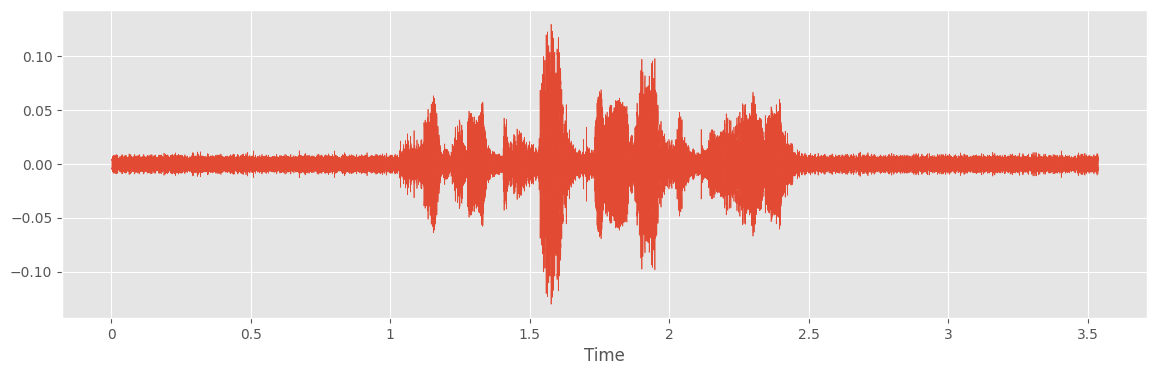
\includegraphics[width=\linewidth]{Noise Surprise.png} 
        \caption{Added noise}
        \label{fig:surprise_noise}
    \end{subfigure}

    \vspace{1em} 

    % Second row
    \begin{subfigure}[t]{0.48\textwidth}
        \centering
        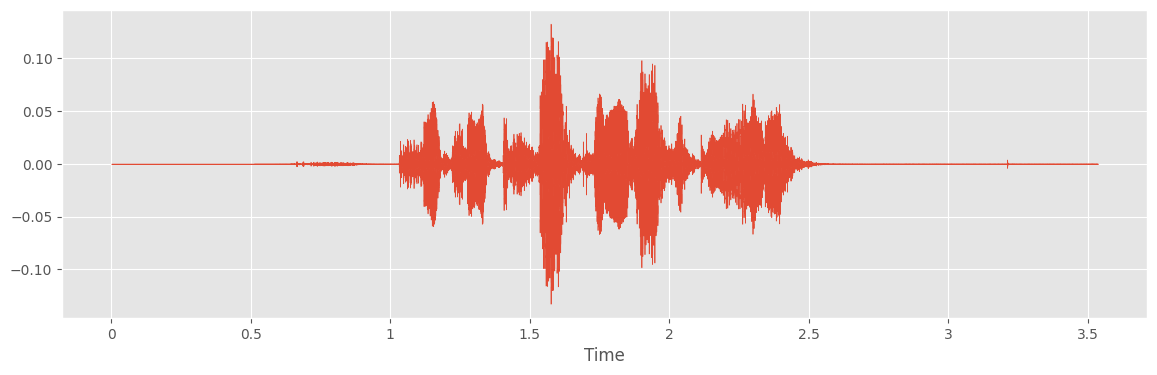
\includegraphics[width=\linewidth]{Pitch Surprise.png} 
        \caption{Pitch bending waveform}
        \label{fig:surprise_pitch}
    \end{subfigure}\hfill
    \begin{subfigure}[t]{0.48\textwidth}
        \centering
        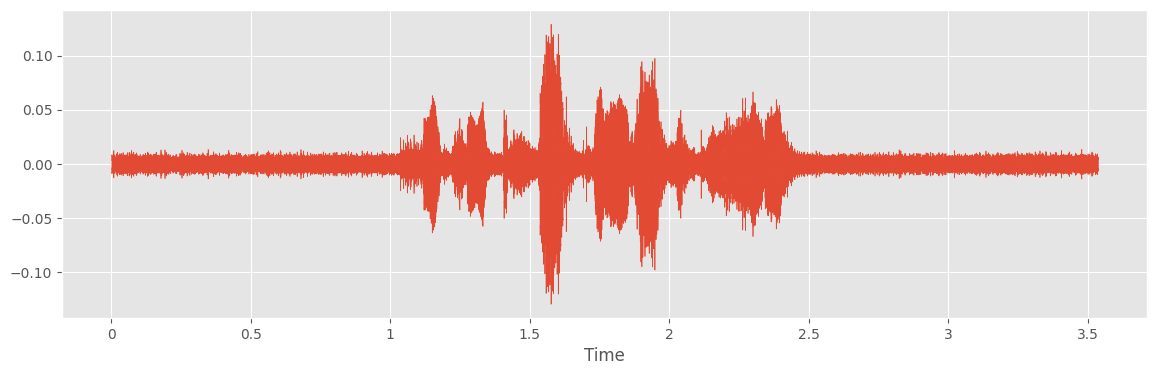
\includegraphics[width=\linewidth]{Mix Surprise.png} 
        \caption{Noise and Pitch bending waveform}
        \label{fig:surprise_mix}
    \end{subfigure}

    \caption{Waveform comparison of Surprise emotion audio sample under different augmentations.}
    \label{fig:surprise_audio_augmentation}
\end{figure}

\subsection{Feature Extraction}\label{subsec3.3}
Feature extraction plays a critical role in transforming raw speech signals into discriminative representations for emotion recognition. In the proposed framework, both acoustic and semantic features are extracted to capture complementary aspects of emotional expression. While acoustic features encode spectral and temporal characteristics of speech, semantic representations provide high-level contextual information derived from learned speech embeddings.

%The feature extraction process forms the base for the emotion recognition system. In this process, we transform the raw preprocessed audio signal into a set of meaningful numerical representations, which serve as an input to a model. In this section, we explore the feature extraction pipeline for a proposed framework. We aim to capture the subtle changes in the speech to understand the emotional state, just like humans do. Based on previously explored and popular emotion recognition and speech signal processing techniques \cite{r3, r4, r5}, we carefully selected and extracted a set of acoustic features and sentiments from the speech.

\subsubsection{Acoustic Features}\label{subsubsec3.3.1}
 To model the low-level properties of speech signals, three widely adopted acoustic descriptors are extracted: Zero Crossing Rate (ZCR), Root Mean Square Energy (RMSE), and Mel-Frequency Cepstral Coefficients (MFCCs). These features are computed on short-time frames to capture temporal variations in speech.
 
\begin{enumerate}

    \item \textbf{Zero Crossing Rate (ZCR):}\\
  ZCR measures the rate of sign changes in the speech signal and provides insight into the frequency characteristics of the audio. It is particularly useful for distinguishing between voiced and unvoiced segments and capturing high-frequency components associated with certain emotional states. For a discrete-time signal 
 $y[n]$ ZCR is defined as:
  \begin{equation}
    ZCR = \frac{1}{2T} \sum_{n=1}^{T} |\text{sgn}(y[n]) - \text{sgn}(y[n-1])|
    \end{equation}
    where sgn(y[n]) is the sign function:
    \begin{equation}
    \text{sgn}(y[n]) =
    \begin{cases}
        1 & \text{if } y[n] > 0 \\
        -1 & \text{if } y[n] < 0 \\
        0 & \text{if } y[n] = 0
    \end{cases}
    \end{equation}
    where T denotes the frame length.
    
    
    
%    The Zero Crossing Rate (ZCR) is a low-level acoustic feature that is used to measure the number of times the amplitude of the speech signal changes from positive to negative or from negative to positive within a specific time frame. It offers information about the spectral characteristics of the speech, like the dominance of high frequencies in an audio signal, which indicates certain emotions like anger or fear \cite{r4}. For each audio sample, 108 ZCR values were computed. The ZCR for a discrete-time signal $y[n]$ of length $T$ within a frame is calculated as:
%    \begin{equation}
 %    ZCR = \frac{1}{2T} \sum_{n=1}^{T} |\text{sgn}(y[n]) - \text{sgn}(y[n-1])|
 %    \end{equation}
%     where sgn(y[n]) is the sign function:
 %    \begin{equation}
 %    \text{sgn}(y[n]) =
 %    \begin{cases}
 %        1 & \text{if } y[n] > 0 \\
  %       -1 & \text{if } y[n] < 0 \\
 %       0 & \text{if } y[n] = 0
%     \end{cases}
 %    \end{equation}
%     The outputs of the sign function are +1 if the sample signal is positive, -1 if the sample signal is negative, and 0 if it's exactly zero. The exact difference between the signs of the samples "$|\text{sgn}(y[n]) - \text{sgn}(y[n-1])|$", is calculated. This difference will be 2 if the sign changes between the two samples (e.g., from positive to negative or vice versa), and 0 if the signs remain the same (both positive, both negative, or both zero). Higher ZCR values indicate faster frequency changes, often associated with noisy signals suggesting emotions like anger or fear. Conversely, lower ZCR indicates smoother energy curves and less high-frequency content, pointing to emotions like sadness or neutral.\\
    
% --------------------------------------------------------------------------------------------

    \item \textbf{Root Mean Square Energy (RMSE):}\\
RMSE represents the short-term energy of the speech signal and reflects variations in speech intensity. Emotional states such as anger and excitement typically exhibit higher energy levels, whereas sadness and neutrality correspond to lower energy. RMSE is computed as:
 \begin{equation}
    RMSE = \sqrt{\frac{1}{T} \sum_{n=1}^{T} y[n]^2}
    \end{equation}    
    
    
    
%    The Root Mean Square Energy (RMSE) measures the average power of the audio signal within a given frame for each audio sample. It calculates the loudness or intensity of the speech, which frequently changes with the intensity of the emotions. For example, emotions like anger may be linked to higher energy levels compared to emotions like sadness, which may be linked to lower energy levels \cite{r4}. For each audio sample, 108 RMSE values were computed. The RMSE for a discrete-time signal $y[n]$ of length $T$ within a frame is computed as:
%    \begin{equation}
 %    RMSE = \sqrt{\frac{1}{T} \sum_{n=1}^{T} y[n]^2}
%     \end{equation}
 %    The calculation is done by taking a discrete-time sample $y[n]$ within the frame, then the values are squared, $(y[n]^2)$ and then these squared values are summed up within the entire frame $\sum_{n=1}^{T} y[n]^2$. This sum represents the total energy within the frame. A higher RMSE value refers to more energetic and louder speech segments.\\

% --------------------------------------------------------------------------------------------

    \item \textbf{Mel-Frequency Cepstral Coefficients (MFCCs):}\\
MFCCs are widely used to model the perceptual characteristics of human hearing. They are obtained by applying a Mel-scaled filter bank to the power spectrum of the signal, followed by logarithmic compression and Discrete Cosine Transform (DCT). This process captures the spectral envelope of speech, which is highly sensitive to emotional variations.

In this work, 20 MFCC coefficients are extracted per frame along with their first- and second-order derivatives (delta and delta-delta features), resulting in a high-dimensional representation that captures both static and dynamic speech characteristics.

    
%    Mel-Frequency Cepstral Coefficients (MFCCs) play a crucial role in speech analysis, they are designed to simulate how the human auditory system perceives sound frequencies. It is extracted by applying a number of changes to each audio frame power spectrum. After the Mel filter bank, which is obtained by applying a collection of triangular filters spaced in line with the Mel scale, which results in logarithmic filter banks energies and then applying the Discrete Cosine Transform (DCT). The overall spectral form is represented by the DCT's lower-order coefficients, which are highly sensitive to subtle changes in tonal representation, which is affected by emotional expressions \cite{r3}.
    
\iffalse 
\noindent Here are the steps for MFCC extraction:
    \begin{itemize}
    
    \item \textbf{Framing}: The continuous audio signal is segmented into multiple overlapping frames. This allows the analysis of the audio signal, capturing information on how the speech changes over a period of time.
    
    \item \textbf{Windowing}: Each overlapping frame segmented is then multiplied by a window function like the Hamming window. This step is crucial because it helps reduce the spectral loss, which is caused by the abruptly segmented frames.
    
    \item \textbf{Fast Fourier Transform (FFT)}: The Fast Fourier Transform (FFT) algorithm computes the frequency spectrum for each windowed frame. The FFT converts the time-domain signal into individual frequencies with their corresponding magnitudes and phases. This output contains a set of bins consisting of a numerical representation of the spectral information of the frame.

    \item \textbf{Power Spectrum Estimation}: The power spectrum is calculated from the FFT bins. The power spectrum displays the distribution of signal energy across different frequencies.

    \item \textbf{Mel Filter Bank Application}: The power spectrum is then passed through banks of triangular bandpass filters spaced based on the Mel scale. The Mel scale is a perception scale of the tone that listeners consider to be equally spaced apart. This outputs filter bank energies containing a set of energies for each band.

    \item \textbf{Logarithm of Filter Bank Energy}: The logarithm of each energy filter bank is computed. This step is motivated by the sensitivity of the human ear to sound intensity.

    \item \textbf{Discrete Cosine Transform (DCT)}: Discrete Cosine Transform (DCT) is applied to the logarithm of the filter bank energies. The DCT eliminates redundant energy values and condenses the signal's spectral properties into a smaller set of coefficients, with the lower ones reflecting the overall shape of the frequency spectrum, which is highly sensitive to changes in the vocal tonal shifts.

    \end{itemize}

    In our study, we extracted a total of 20 MFCCs for each frame, representing the structure of the signal frequency. We also computed the first derivatives and second derivatives of the MFCCs. Resulting in a future vector of size 2160, which was obtained from each audio sample. The first derivatives of the MFCCs represent the speed and direction of MFCCs. The delta will be a large positive if the value is increasing rapidly, a small negative number if the value is decreasing slowly, and close to zero if the value stays the same. The second derivative tells us about the acceleration and deceleration of the change itself: a large positive number if the rate of change is increasing rapidly and a small negative number if the rate of change is slowing down. 
 \fi   


\end{enumerate}

\subsubsection{Sentiment Features}\label{subsubsec3.3.2}
In addition to acoustic features, high-level semantic representations are extracted using a pre-trained HuBERT model fine-tuned for speech emotion recognition. These embeddings capture contextual and linguistic information that may not be explicitly represented in handcrafted features.

Each audio sample is resampled to 16 kHz and passed through the pre-trained model to obtain a fixed-dimensional embedding representing the underlying emotional context. Unlike traditional sentiment classification outputs, these embeddings provide richer and continuous representations of emotional semantics.
\subsubsection{Feature Fusion}\label{subsubsec3.3.3}
The final feature vector is constructed by concatenating acoustic features (ZCR, RMSE, MFCCs and their derivatives) with semantic embeddings obtained from the HuBERT model. This hybrid representation enables the model to jointly learn from both low-level signal characteristics and high-level contextual information, leading to improved emotion discrimination.


\iffalse  
Apart from traditional acoustic features, we also extracted sentiments by leveraging a pre-trained model for audio sentiment classification. This approach recognizes that the perceived emotion in the speech can also be affected by linguistic content. The \href{https://huggingface.co/superb/hubert-base-superb-er}{Hubert Base Superb Er} model is a powerful tool for emotion recognition in speech. Built on the hubert-base-ls960 model, it's been fine-tuned for the SUPERB Emotion Recognition task \cite{r17}. This model can classify emotions into four categories and is designed to work with 16 kHz sampled speech audio. The pre-trained model takes audio samples as input and outputs a predefined set of sentiment categories (e.g., 'anger,' 'happy,' 'neutral,' 'sad'). We fed the pre-trained sentiment classifier each audio utterance in our dataset after resampling it to the model's required sampling rate (16000 Hz). The result was a single sentiment from the predefined category. The output was then label encoded, creating a vector of 1's and 0's, where the 1 represented the classified sentiment by the pretrained model and the 0's showed other sentiments from the predefined category; for example, the vector [0, 0, 1, 0] displayed neutral sentiment. This enables our primary emotion recognition model to gain from the pre-trained sentiment model's high-level emotional understanding.

\fi

\subsection{Deep Learning Model}\label{subsec3.4}

To model the complex relationship between extracted features and emotional states, a deep learning-based classification approach is adopted. Specifically, a one-dimensional Convolutional Neural Network (1D-CNN) architecture is designed to effectively capture temporal dependencies and hierarchical feature representations from sequential speech data.

As illustrated in Fig. 4, the proposed architecture consists of five stacked Conv1D layers. Unlike two-dimensional convolution, which operates on spatial data, 1D convolution is well-suited for sequential inputs such as time-series speech features, enabling efficient modeling of temporal patterns.

Each Conv1D layer is followed by batch normalization, Rectified Linear Unit (ReLU) activation, and max-pooling operations. Batch normalization is employed to stabilize training and accelerate convergence by normalizing intermediate feature distributions. Max-pooling, with a pool size of 5 and stride of 2, is used to progressively reduce feature dimensionality, thereby lowering computational complexity and mitigating overfitting.

The convolutional layers are configured with decreasing filter sizes to enable hierarchical feature abstraction. The first and second layers contain 512 filters each, followed by two layers with 256 filters, and a final layer with 128 filters. This progressive reduction allows the network to transition from low-level feature extraction to high-level representation learning.

The output of the final convolutional block is flattened and passed to a fully connected (dense) layer with 512 units and ReLU activation, which captures higher-level interactions among extracted features. Finally, the output layer consists of a dense layer with seven units corresponding to the emotion classes, followed by a softmax activation function to produce class probabilities.The softmax function is defined as:
\begin{equation}
\text{Softmax}(\mathbf{z})_i = \frac{e^{z_i}}{\sum_{j=1}^{K} e^{z_j}}
\end{equation}
where  $z_i$ is the logit  for the $i^{th}$ class and $K$ is the number of classes.The output of the softmax layer is a probability distribution over all emotion categories, and the class with the highest probability is selected as the predicted emotion.










\iffalse
For our proposed framework, we employed a deep learning-based classification technique, which effectively helped to learn the complex relationship between the extracted feature and the expressed emotion. We designed and implemented a one-dimensional Convolutional Neural Network (Conv1D) architecture, refer to Figure \ref{fig:Conv1d_Architecture}. Conv1D is a modified type of 2D CNN that can process one-dimensional sequential data, such as text or time series. It has achieved remarkable success in understanding hierarchical data, making it well suitable for analyzing time-series features like those extracted from speech signals.

\begin{figure*}[h]
\centering
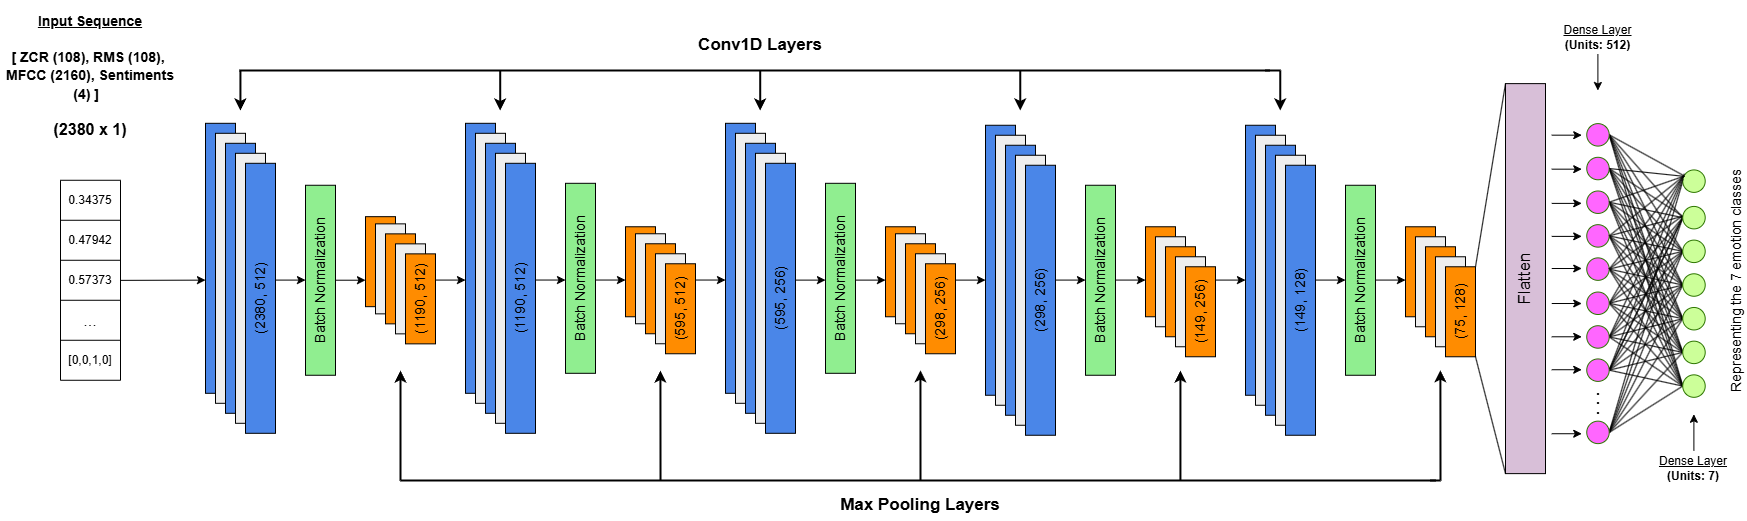
\includegraphics[width=\textwidth]{1D CNN Exploded View_New (1).png}
\caption{Proposed speech emotion recognition model}
\label{fig:Conv1d_Architecture}
\end{figure*}

Our model architecture consists of five Conv1D layers arranged sequentially with a rectified linear unit (ReLU) activation to extract and learn salient features from the input sequence. Each Conv1D layer is followed by a batch normalization layer and a max pooling layer. The batch normalization layer is employed to make the neural network train faster and more stable by normalizing the input layer through re-scaling and re-centering. The max pooling layer, with a pool size of 5 and a stride of 2, reduces the spatial dimensionality of the feature by down-sampling it, making our model less prone to overfitting, improving generalization and reducing the computational requirement. The first and second Conv1D layers have 512 units, the third and fourth Conv1D layers have 256 units, and the fifth Conv1D layer has 128 units. After this the features were fed into a dense (fully connected) layer with 512 units and ReLU activation; this layer was employed to learn a higher-level representation from the extracted features. Lastly, the output layer consists of a fully connected dense layer with 7 units and a softmax function, representing the range of seven emotional categories in our dataset.
\begin{equation}
\text{Softmax}(\mathbf{z})_i = \frac{e^{z_i}}{\sum_{j=1}^{K} e^{z_j}}
\end{equation}
\noindent Where:
\begin{itemize}
    \item $z_i$ is the logit (the output of the previous layer in the network) for the $i^{th}$ class.
    \item $K$ is the number of classes.
    \item $e^{z_i}$ represents the exponential of the logit.
    \item $\sum_{j=1}^{K} e^{z_j}$ is the sum of exponentials across all classes.
\end{itemize}
\noindent The softmax activation function was applied to the output of this layer, which returns a probability distribution over the seven different emotion classes. The emotion with the highest probability was considered the model's prediction for the input utterance.

\fi

\subsection{Evaluation Metrics}\label{subsec3.5}

To evaluate the performance of the proposed speech emotion recognition (SER) system, standard classification metrics are employed. Given the multi-class nature of the problem and potential class imbalance, both overall and class-wise evaluation measures are considered.

\begin{enumerate}
  
    \item \textbf{Accuracy}: Accuracy measures the proportion of correctly classified samples among all predictions and is defined as:
         \begin{equation}
             \text{Accuracy} = \frac{\text{No. of Correct Predictions}}{\text{Total number of Predictions}}
        \end{equation}
     \item \textbf{Precision,Recall, and F1-Score}:
    To assess class-wise performance, precision, recall, and F1-score are computed for each emotion class:
    \begin{equation}
        \text{Precision} = \frac{\text{True Positives}}{\text{True Positives} + \text{False Positives}}
     \end{equation}
    \begin{equation}
        \text{Recall} = \frac{\text{True Positives}}{\text{True Positives} + \text{False Negatives}}
    \end{equation}
     \begin{equation}
        \text{F1-Score} = 2 \times \frac{\text{Precision} \times \text{Recall}}{\text{Precision} + \text{Recall}}
    \end{equation}
         
    These metrics are particularly important in multi-class classification scenarios, where they provide a balanced evaluation of the model’s ability to correctly identify and distinguish between different emotional states. Macro-averaging is used to ensure equal importance across all classes.

     \item \textbf{Confusion Matrix}: A confusion matrix is utilized to provide a detailed visualization of classification performance across all emotion categories. It highlights both correctly classified instances (diagonal elements) and misclassifications (off-diagonal elements), enabling deeper analysis of inter-class confusion patterns.
    
\end{enumerate}



\iffalse  
To evaluate the performance of our proposed emotion recognition system, we employed various metrics widely used in the classification field. The metric provides a detailed understanding of the model's ability to accurately recognize different emotional states in speech. The metrics used in our proposed method are

\begin{enumerate}
    \item \textbf{Accuracy}: It is a fundamental metric evaluating the performance of the classification model. It measures how well the model is predicting labels for unseen data. It is calculated as follows:
    \begin{equation}
    \text{Accuracy} = \frac{\text{No. of Correct Predictions}}{\text{Total number of Predictions}}
    \end{equation}
    On the testing set, our model has achieved an accuracy of \textbf{96.56\%} which shows a high level of correlation between the prediction and the true emotional labels, suggesting that our model has effectively learned the underlying patterns corresponding to each emotional state in the speech.\\
    
    \item \textbf{Precision, Recall, and F1-Score}: To gain more understanding about our model's performance for each emotional class, we calculated precision, recall and F1-score, which are important in multi-class classification tasks and especially when dealing with class imbalance.

    \begin{itemize}
        \item \textbf{Precision}: It is a measure of a model's performance that tells you how often the prediction made by the model is actually correct. It is calculated as follows:
        \begin{equation}
        \text{Precision} = \frac{\text{True Positives}}{\text{True Positives} + \text{False Positives}}
        \end{equation}
        True Positive (TP) represents correctly predicted instances of the actual class, and False Positives (FP) reflect instances that were incorrectly predicted.\\
        
        \item \textbf{Recall}: Recall (also known as sensitivity) provides a proportion of correctly predicted positive instances out of all actual positive cases. It is calculated as follows:
        \begin{equation}
        \text{Recall} = \frac{\text{True Positives}}{\text{True Positives} + \text{False Negatives}}
        \end{equation}
        False Negatives (FN) are the instances that were incorrectly classified as another class.\\
        
        \item \textbf{F1-Score}: F1-Score is a harmonic mean between recall and precision. The metric tells us how accurate (identifies the number of instances properly) and robust (does not miss any significant number of instances) our model is. It provides a balanced measure of model performance, especially when dealing with imbalanced classes in a dataset. The mathematical expression for F1-Score is as follows:
        \begin{equation}
        \text{F1-Score} = 2 \times \frac{\text{Precision} \times \text{Recall}}{\text{Precision} + \text{Recall}}
        \end{equation}
        Higher precision and lower recall can give you higher accuracy but miss a large number of instances.
        
    \end{itemize}
    
    \item \textbf{Confusion Matrix}: Confusion matrix creates a ${N X N}$ matrix, where N is the number of classes or categories that are to be predicted. The confusion matrix visually provides a detailed description of the model's performance, showing the number of instances the model correctly classified each emotion and the number of instances where it misclassified one as another emotion. Each row of the matrix represents the actual emotion, while each column represents the predicted emotion. The diagonal elements show the correctly classified instances and the off-diagonal elements show the misclassified instances.
    \begin{itemize}
        \item True Positive (TP): The number of instances where the model correctly predicted the positive class.
        \item True Negative (TN): The number of instances where the model correctly predicted the negative class.
        \item False Positive (FP): The number of instances where the model incorrectly predicted the positive class.
        \item False Negative (FN): The number of instances where the model incorrectly predicted the negative class.
    \end{itemize}

\end{enumerate}
\fi
\section{Discussion and Results}\label{sec4}
This section presents the experimental evaluation of the proposed Speech Emotion Recognition (SER) framework. The objective is to assess the effectiveness of the model in accurately classifying emotional states from speech signals under diverse conditions.

The model was trained using the RMSProp optimization algorithm, which is widely adopted for its ability to provide stable and efficient convergence in deep learning models. The key hyperparameters used during training, including learning rate, batch size, number of epochs, and regularization strategies, are summarized in Table \ref{tab:model_config}. To ensure reproducibility, all experiments were conducted under consistent training conditions. 

\iffalse
This section presents a comprehensive analysis of our experiments, achieved from our speech emotion recognition system (SER). We detail the parameters used in our experimentation, followed by stating the performance scores obtained from our proposed 1D convolutional model on the testing set. Lastly, we will discuss the findings and compare them with relevant literature in the field.

\subsection{Experiment Settings}\label{subsec4.1}
In the proposed method we employed RMSProp (Root Mean Square Propagation), a widely used optimization algorithm in deep learning, to make sure that our results are consistent and can be reproduced. The key parameters that were used to design the experimentation are summarized in 
\fi
Table \ref{tab:model_config}.

\begin{table*}[h]
\caption{Experimentation Parameters}\label{tab:model_config}
\centering
\normalsize
\begin{tabular}{@{}l | p{0.5\textwidth}@{}}
\toprule
\textbf{Parameter} & \textbf{Value} \\
\midrule
Learning Rate & Initial 0.001 (RMSprop default),\\ 
& Scheduled reduction with factor 0.5 \\ 
\midrule
Number of Epochs & 50 (Early stopping with patience = 5) \\
\midrule
Batch Size & 64 \\
\midrule
Activation Function & ReLU, Softmax (output) \\
\midrule
Optimization Algorithm & RMSprop \\
\midrule
Hyperparameter Optimization & Learning rate scheduling, Early stopping \\
\bottomrule
\end{tabular}
\end{table*}

\subsection{Model Evaluation}\label{subsec4.2}
The performance of the proposed model was evaluated on a held-out test set consisting of 12,290 audio samples. The evaluation metrics include accuracy, precision, recall, and F1-score, as summarized in Table \ref{tab:model_performance}.

The model achieved an overall accuracy of 96.56 \%, demonstrating strong generalization capability on unseen data. Additionally, the model attained a precision of 0.9654, recall of 0.9636, and F1-score of 0.9645, indicating a balanced performance with minimal false positives and false negatives.

A detailed class-wise evaluation is presented in Table \ref{tab:classification_report}. The classification report shows consistently high precision, recall, and F1-scores across all seven emotion categories. The macro-average and weighted-average F1-scores are both approximately 0.97, highlighting the robustness and stability of the proposed model across different emotional classes.

Fig. \ref{fig:cm_test} illustrates the confusion matrix for the test set. The dominance of high values along the main diagonal indicates that the majority of samples are correctly classified. Minor confusion is observed between acoustically similar emotion pairs; however, the model maintains strong discriminative capability overall. Notably, even for underrepresented classes such as surprise, the model achieves reliable classification performance, demonstrating its robustness across varying data distributions.

\iffalse
The proposed model was evaluated based on the testing set that comprises of 12,290 audio samples. The overall evaluation result of the model in terms of accuracy, precision, recall and F1-score is given below in Table 
\fi
\ref{tab:model_performance}.

\begin{table*}[h]
\caption{Performance Metrics on Test Data}\label{tab:model_performance}%
\centering
\normalsize
\begin{tabular}{@{}lcccc@{}} 
\toprule
\textbf{Model} & \textbf{Accuracy} & \textbf{Precision} & \textbf{Recall} & \textbf{F1-Score} \\
\midrule
Conv1D & 96.56\% & 96.54\% & 96.36\% & 96.45\% \\
\bottomrule
\end{tabular}
\end{table*}
\iffalse
This indicates that our model achieved high accuracy of 96.56\% on unseen test samples, showing a great ability for generalization. Additionally, metrics like the F1-score of 0.9645, precision of 0.9654 and recall of 0.9636 show the robustness of the model, minimizing both false positives and false negatives.

The classification report shows the model's high precision, recall, and F1-scores across all seven emotion classes; refer to Table \ref{tab:classification_report}. The macro-average and weighted-average F1-scores of \textbf{0.97}, proving the model's reliability and consistency in performance across all emotional categories.
\fi


\begin{table*}[h]
\caption{Classification Report}\label{tab:classification_report}%
\centering
\normalsize
\begin{tabular}{@{}lcccc@{}}
\toprule
& \textbf{precision} & \textbf{recall} & \textbf{f1-score} & \textbf{support} \\
\midrule
angry & 0.96 & 0.97 & 0.97 & 1896 \\
disgust & 0.97 & 0.96 & 0.96 & 1811 \\
fear & 0.96 & 0.96 & 0.96 & 1870 \\
happy & 0.96 & 0.96 & 0.96 & 2157 \\
neutral & 0.96 & 0.97 & 0.97 & 1822 \\
sad & 0.97 & 0.97 & 0.97 & 1884 \\
surprise & 0.98 & 0.96 & 0.97 & 850 \\
\midrule
accuracy & & & 0.97 & 12290 \\
macro avg & 0.97 & 0.97 & 0.97 & 12290 \\
weighted avg & 0.97 & 0.97 & 0.97 & 12290 \\
\bottomrule
\end{tabular}
\end{table*}

\iffalse
The performance of classification across the seven emotions on the texting dataset can be seen in Figure \ref{fig:cm_test}. It shows a high value of predictions along the main diagonal. Especially, the model shows a high number of accurate predictions with minimal confusion with other emotions, even though the "surprise" category has fewer samples, reflecting the model's robustness and the ability to correctly predict in most acoustic settings. 
\fi
\begin{figure}[h]
\centering
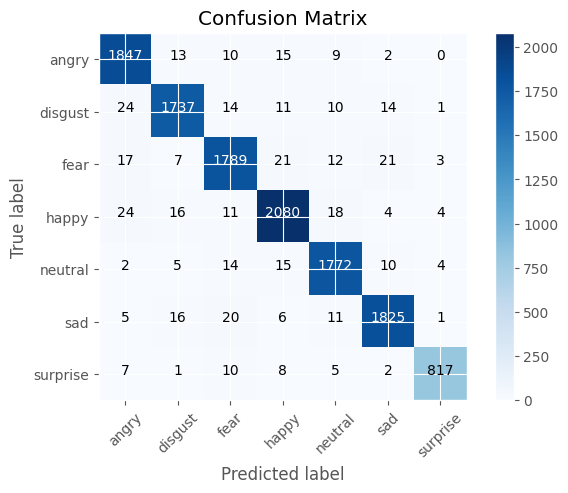
\includegraphics[width=\linewidth]{Confusion_matrix.png}
\caption{Confusion matrix plot on unseen audio samples for our proposed framework.}
\label{fig:cm_test}
\end{figure}

\subsection{Performance Comparison with Existing Literature}\label{subsec4.3}
This section presents a comparative study of the accuracy achieved by our proposed CNN-1D model with existing methods in speech emotion recognition, shown in Table \ref{tab:accuracy_comparison}. Compared to other studies, our proposed model was trained on a variety of datasets, including CREMA-D, RAVDESS, Hindi, TESS, and SAVEE, which introduces more diversity and contributed to a higher accuracy of 96.56\%. Traditional models like Gaussian Mixture Models (GMM) by Kandali et al. (2008) \cite{r11} and Support Vector Machines (SVM) by Shen et al. (2011) \cite{r12} achieved accuracies of 76.50\% and 82.50\%, respectively, highlighting the achievement in machine learning methods. 

Recent advancements in deep learning architectures like 1D CNN by Li et al. (2019) \cite{r13} on the RAVDESS dataset (76\%), and Long Short-Term Memory (LSTM) networks by Chopra et al. (2021) \cite{r14} across multiple datasets (67\%), show a considerable performance gap compared to our results. Even comparing with studies incorporating attention mechanisms, such as CNN + Attention by Peng et al. (2020) \cite{r15} on IEMO-CAP (76.36\%) and LSTM + Attention + CNN-2D by Singh et al. (2023) \cite{r16} on RAVDESS (74.44\%), our model considerably outperformed them.

\begin{table*}[h]
\caption{Accuracy comparison with relevant literature studies.}\label{tab:accuracy_comparison}
\centering
\normalsize 
\begin{tabular}{@{} p{0.15\linewidth} | p{0.2\linewidth} | p{0.25\linewidth} | c @{}}
\toprule
\textbf{Model} & \textbf{Reference} & \textbf{Dataset Used} & \textbf{Accuracy Percentage} \\
\midrule
GMM & Kandali et al. (2008) \cite{r11} & Custom Recorded & 76.50\% \\
\addlinespace
SVM & Shen et al. (2011) \cite{r12} & Berlin & 82.50\% \\
\addlinespace
CNN-1D & Li et al. (2019) \cite{r13} & RAVDESS & 76\% \\
\addlinespace
CNN + Attention & Peng et al. (2020) \cite{r15} & IEMO-CAP & 76.36\% \\
\addlinespace
LSTM & Chopra et al. (2021) \cite{r14} & RAVDESS, TESS, EMODB, SAVEE  & 67\% \\
\addlinespace
LSTM + Attention + CNN-2D & Singh et al. (2023) \cite{r16} & RAVDESS & 74.44\% \\
\midrule
\textbf{CNN-1D} & \textbf{PROPOSED} & TESS, CREMA-D, SAVEE, HINDI, RAVDESS  & \textbf{96.56\%} \\
\bottomrule
\end{tabular}
\end{table*}


\section{Conclusion}\label{sec5}
In this research work, we present a detailed study about speech emotion recognition that leverages 1D-CNN that was trained on a large and diverse speech corpus, which was achieved by performing data augmentation techniques. We also extracted a wide range of acoustic features like ZCR, RMS, and MFCCs and, importantly, sentiments, which were derived using a pre-trained HuBert model. These features were arranged in proper order and were fed as input to the 1D CNN architecture that was optimized for learning temporal patterns and classifying from a range of seven emotional expressions (Anger, Disgust, Fear, Happy, Neutral, Sad, and Surprise). 

The proposed framework displayed efficiency by achieving high accuracy of 96.56\% on the testing set. Additionally, the classification report also displayed important evaluation metrics like precision, recall and F1-score across all seven emotions, which indicated the robustness and the ability to generalize. 

Comparing our model with the recent studies in the field highlighted the performance improvement of our proposed model, outperforming complex architectures that incorporated techniques like attention mechanisms. This suggests that the complex features of emotional expression and subtle shifts in tone in speech can be captured by using a well-tuned 1D CNN when combined with  a broad feature set consisting of acoustic features of the audio signal and sentiments from the linguistic content of the speech.

In conclusion, this study demonstrated the model's excellent performance, which was attributed to the integration of sentiment features and the use of a large and diverse dataset. These results pave the way for more research into various efficient deep learning architectures and feature engineering techniques to understand the emotional content of human speech and provide insightful information to the field.

%% ============================================================================================
%% Declarations

\section*{\normalsize Compliance with Ethical Standards}

\subsection*{\small Author Contributions \\
{\normalfont{\small Shubham Vankalas: Conceptualization, Methodology, Data Curation, Writing – Original Draft.}\\
{\small Vandana Dhingra: Methodology, Formal Analysis, Writing – Review \& Editing, Supervision, Validation.}}}
\subsection*{\small Funding: {\normalfont This research received no specific grant from any funding agency in the public, commercial, or not-for-profit sectors.}}
\subsection*{\small Data Availability: {\normalfont The datasets analyzed during the current study are publicly available.}}


\vspace{0.2cm}
\section*{\normalsize Declarations}

\subsection*{\small Conflict of Interest: {\normalfont On behalf of all authors, the corresponding author states that there is no conflict of interest.}}
\subsection*{\small Research Involving Humans and/or Animals: {\normalfont Not applicable.}}
\subsection*{\small Informed Consent: {\normalfont Not applicable.}}
\subsection*{\small Competing Interests: {\normalfont The authors declare that they have no competing interests.}}


\vspace{0.2cm}
\bibliography{sn-bibliography}% common bib file
%% if required, the content of .bbl file can be included here once bbl is generated
%% \input sn-article.bbl

\end{document}
